\title{Distributed Systems II}
\author{Brae Webb}
\date{\week{6}}

\maketitle

\section{Introduction}
In the previous course notes \cite{distributed1-notes} and lecture \cite{distributed1-slides} on distributed systems,
we explored how to leverage distributed systems to increase the reliability and scalability of a system.
Specifically, we saw that when working with stateless services, which do not require persistent data,
auto-scaling groups and load-balancers can be used to scale-out the service --- distributing the load to arbitrary copies of the service.
In the lecture, we applied this technique to the product browsing service of our Sahara example,
as illustrated in Figure \ref{fig:scaled-sahara}.

\begin{figure}[H]
\begin{center}
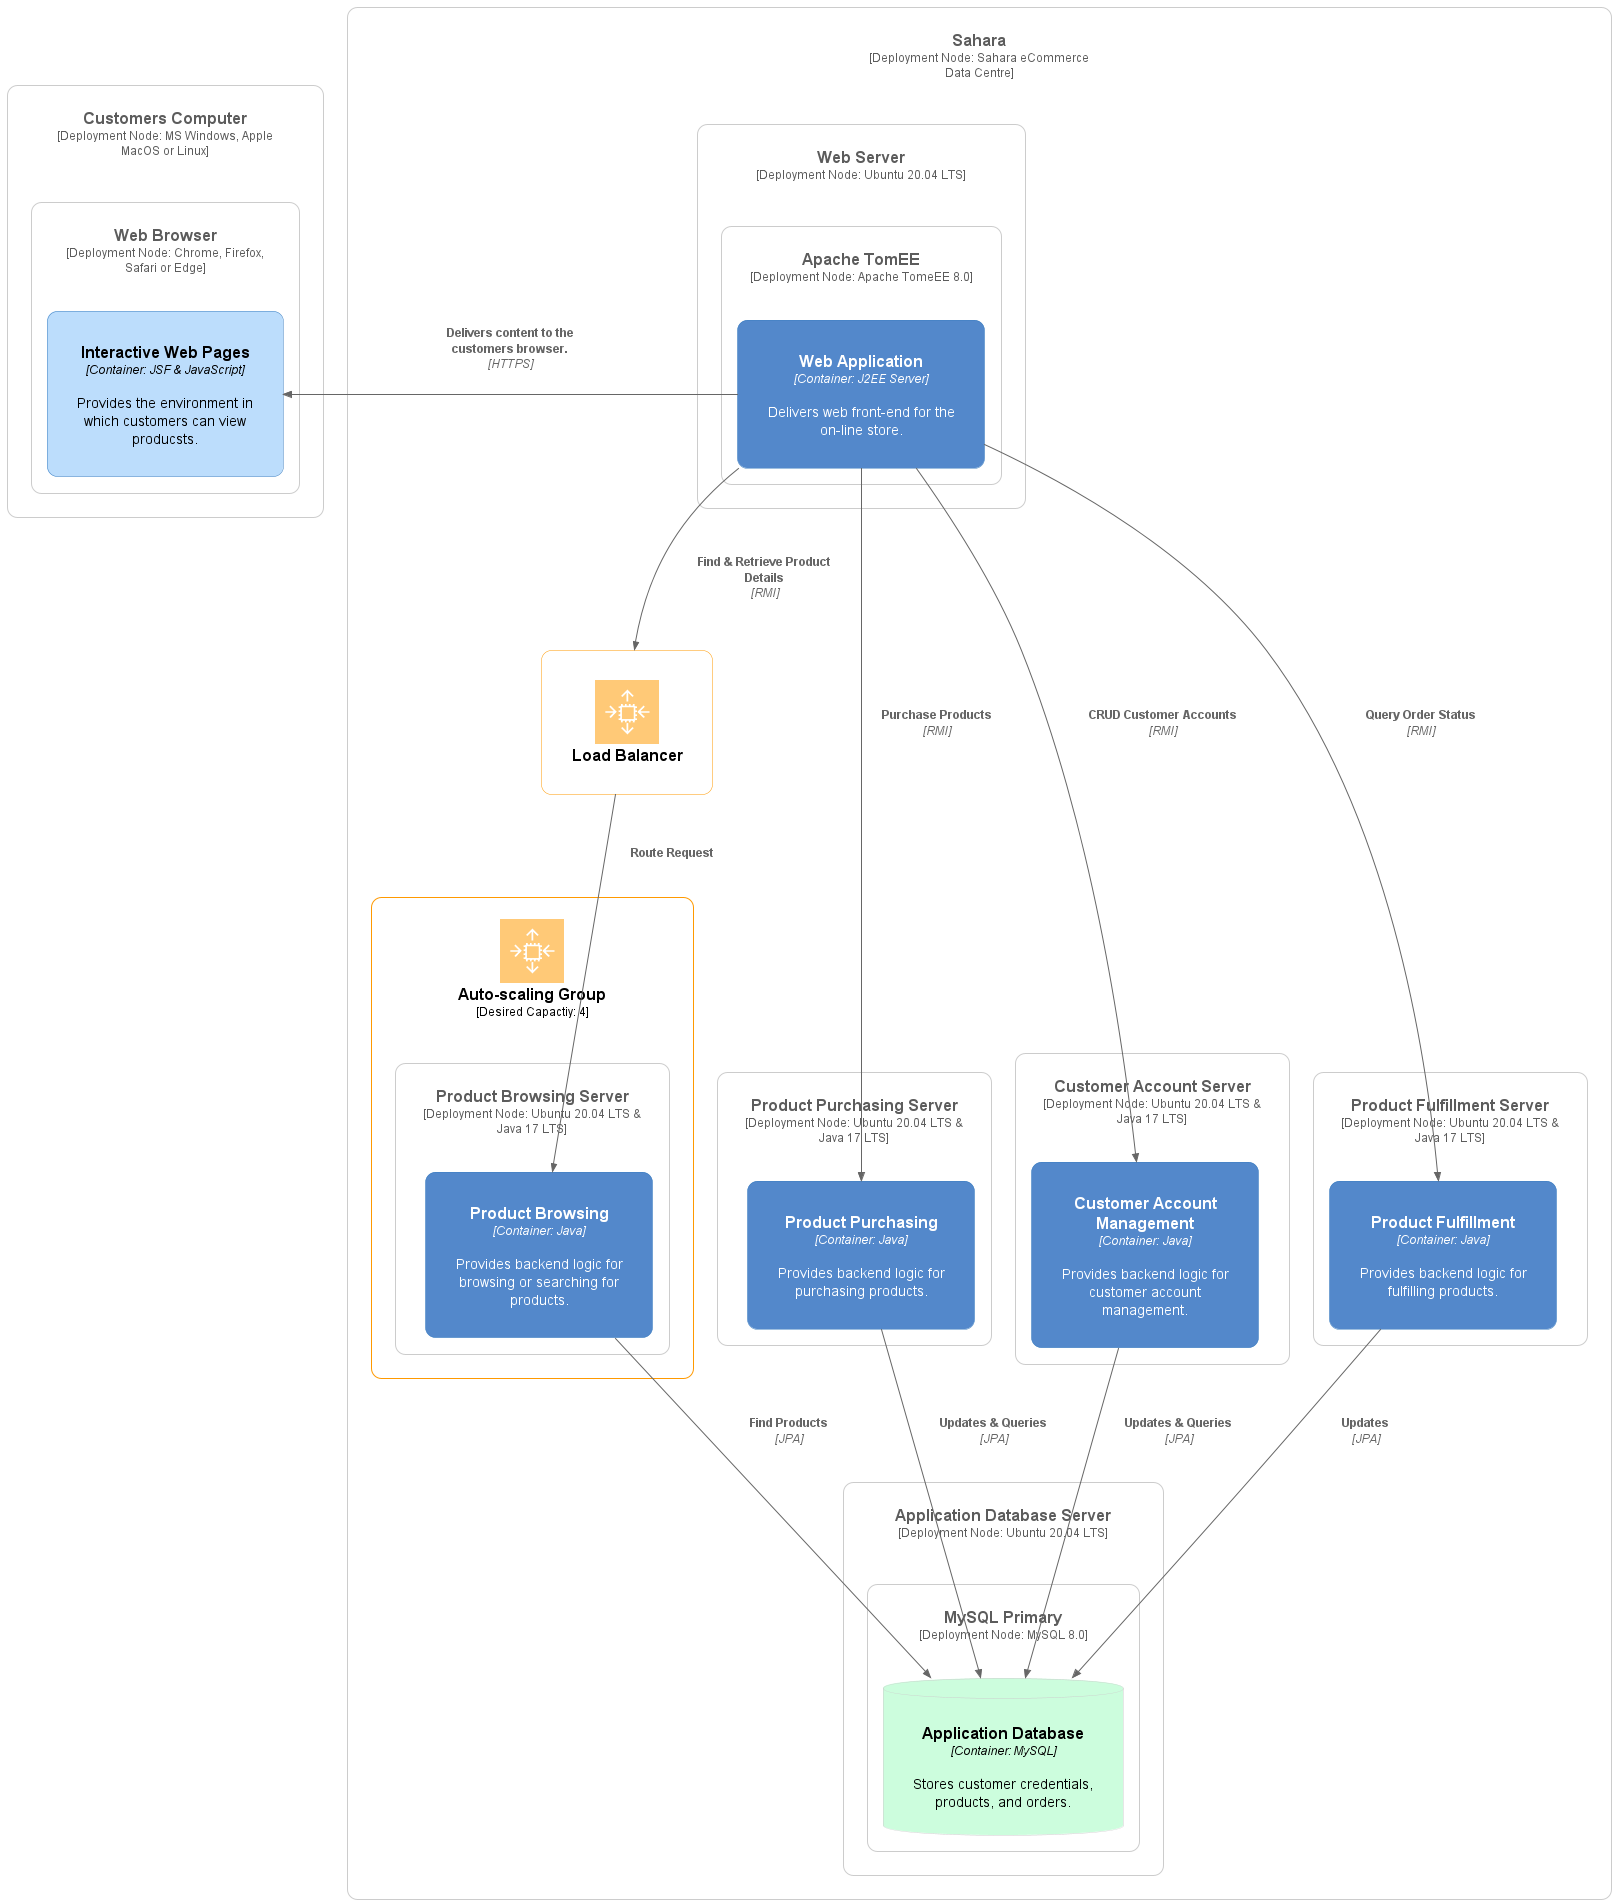
\includegraphics[width=0.72\textwidth]{diagrams/SaharaScaled}
\end{center}
\caption{A service-based implementation of Sahara with stateless scaling techniques applied to the product browsing service.}
\label{fig:scaled-sahara}
\end{figure}

One might correctly identify that by scaling the product browsing service,
we have only increased the maximum load that the database can expect.
The database becomes a major bottle-neck.
We might attempt to scale-up the database,
purchasing more powerful machines to host the database on,
but this approach is limited.

In this part of our distributed systems series,
we look at how to scale stateful services which \textsl{do} require persistent data.
We focus on state stored in a database and thus,
how databases can be made more reliable and scalable.
In these lecture notes we only outline the scope of our treatment of database scaling.
For a detailed treatment of these topics,
please refer to the \textit{Designing Data-Intensive Applications} textbook \cite{data-intensive}.

\section{Replication}
Replication is the most straight-forward approach to scaling databases.
In many applications, read operations occur much more frequently than write operations,
in such cases replication can enable improved capacity for read operations whilst keeping the write capacity roughly equivalent.
Replication involves creating complete database copies, called replicas,
that reduce the load on any single replica.

\subsection{Leader and Followers}
The most common implementation of replication is leader-follower replication.
Fortunately, it is also the simplest.

\begin{description}
    \item[Leader] a replica that accepts write operations and defines the order in which writes are applied.
    \item[Follower] replicas that are read-only copies of the data. 
\end{description}

\noindent
When writes occur, they must be sent to the leader replica.
Leader replicas propagate updates to all followers.
Read operations may occur on any of the follower replicas.

For our example,
we might create two followers, or read replicas,
of the Sahara database.
As the product browsing service is likely to primarily perform read queries,
it may send those requests to one of the read replicas.
Write operations, which are likely to be the majority for the product purchasing service,
must still be sent to the lead replica%
\footnote{Realistically, queries would be forwarded based on their type rather than their service of origin.}.
The resulting system might look like Figure \ref{fig:sahara-leader-follower}.

\begin{figure}[H]
    \begin{center}
    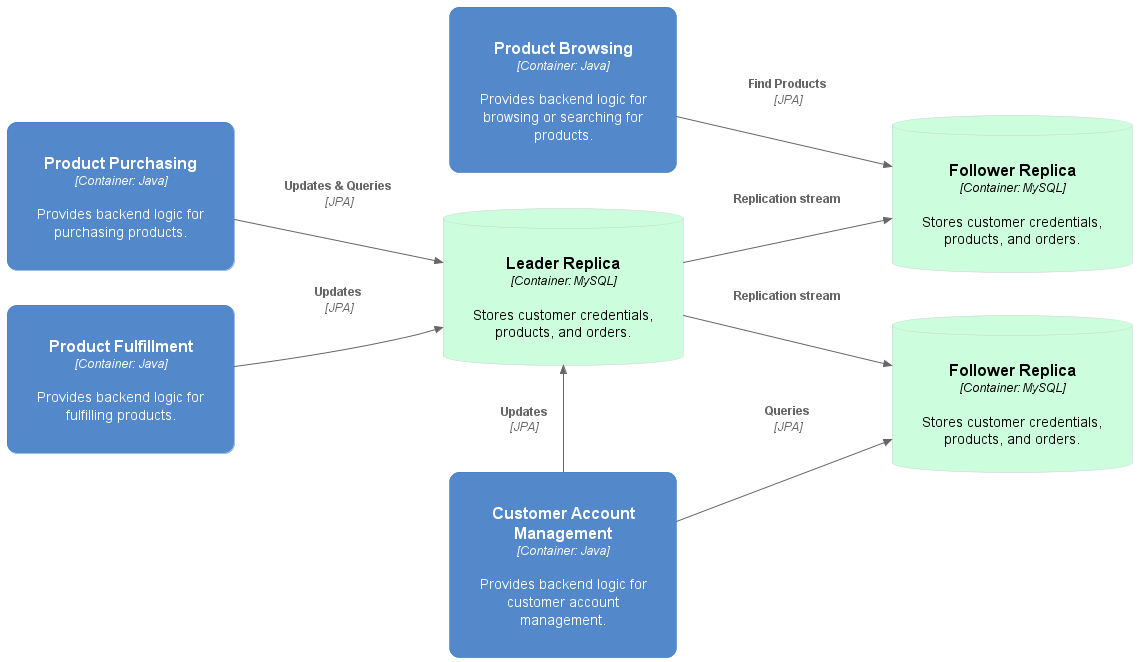
\includegraphics[width=0.9\textwidth]{diagrams/LeaderFollowerSpread}
    \end{center}
    \caption{A leader-follower replication of the Sahara database.}
    \label{fig:sahara-leader-follower}
\end{figure}

\subsubsection*{Replication Lag}

For leader-follower replication to be practical,
write updates from the leader to the followers need to be \textsl{asynchronous}%
\footnote{We need not wait for writes to propagate to all followers before accepting that a write has succeeded}.
However, asynchronous propagation introduces an entirely new suite of issues.
If we do not wait for write updates to be propagated to all replicas,
then there will be times where the data retrieved from a read replica will be out-dated, or \textsl{stale}.
Eventually, all writes will be propagated to every read replica,
so we call this an \textsl{eventually consistent} system.

We have grown fairly accustomed to eventually consistent systems.
Consider the last time you or a friend of yours updated their display picture.
Did everyone start seeing the updated picture immediately, or,
did it take a number of hours or even days to propagate through?
Despite our increased exposure to eventually consistent systems,
there are a few common practices to keep in mind when implementing such a system to preserve your users sanity.

\begin{description}
    \item[Read-your-writes Consistency] Ensures that the user who wrote the database change will always see their update reflected, though other users will still have to wait for the change to be propagated. This type of consistency avoids upsetting users and making them think they must redo their write.
    \item[Monotonic Reads] Ensures that once a user reads the updated data, they do not later see the older version of the data, i.e. they do not travel back in time.
    \item[Consistent Prefix Reads] Ensures that sequential writes are always read in the same order. Consider a Twitter feed, each post is a write. Consistent Prefix Reads guarantees that those readers do not see the posts out of order.
\end{description}

\subsection{Multi-leader Replication}

Leader-follower replications are sufficient for most use cases as reads often occur far more frequently than writes.
However, there are situations where leader-follower replication is insufficient.
For systems which need to be highly available,
having a single point of failure,
the leader replica, is not good enough.
Likewise, for systems which need to be highly scalable,
a write bottle-neck is inappropriate.
For these situations, a multi-leader replication scheme may be appropriate.
It is worth noting that multi-leader replications introduce complexity that often outweighs their value.

\begin{figure}[ht]
    \begin{center}
    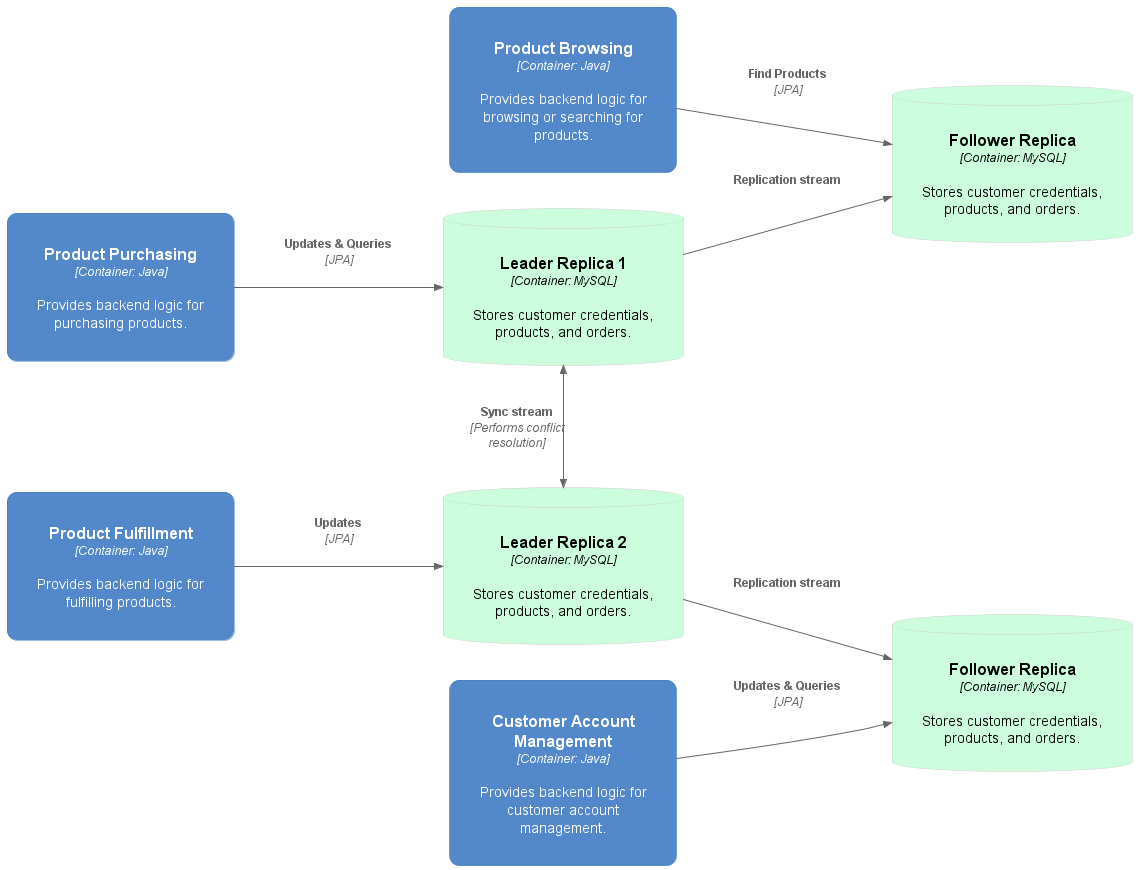
\includegraphics[width=0.8\textwidth]{diagrams/MultiLeader}
    \end{center}
    \caption{A multi-Leader replication of the Sahara database.}
    \label{fig:sahara-multi-leader}
\end{figure}

For our example,
we might naively introduce a system such as Figure \ref{fig:sahara-multi-leader}.
Here we have introduced a second leader,
and each leader has their own follower.
This type of separation might make sense.
We might find it beneficial to have a separate database replica in the warehouse which can be interacted with via the fulfillment service.
Such a system would isolate the warehouse operations team from the potential latency of the external customer load.

However, we now have a system where writes can occur in parallel.
This can cause several problems.
Consider a situation where the fulfillment center has noticed a defective \href{https://www.amazon.com.au/dp/B09LYDDDR1}{Nicholas Cage Reversible Pillow}.
They promptly update their system to reflect the decreased stock.
However, at around the same time,
the CSSE6400 tutors placed a bulk order for all of Sahara's remaining stock.
Both write operations appear successful to the fulfillment team and the tutors but a conflict has occurred --- this is known as a \textsl{write conflict},
and it is a common problem in multi-leader replications. 

\subsubsection*{Write Conflicts}
Write conflicts occur when two or more leaders in a multi-leader replication update the same piece of data.
In relational systems this is normally the same table row.
There are a few mechanisms for resolving write conflicts,
but the recommended approach is to avoid conflicts altogether.
Conflicts can be avoided by ensuring that a piece of data is only ever updated by the same leader,
for example, we might implement that all Nicholas Cage related products are written to Leader Replica 1.

If we are not fortunate enough to be in a situation where conflicts can be avoided,
there are a few techniques we can use.

\begin{itemize}
    \item Assign IDs to writes, and decide which conflicting write to accept based on the ID via some strategy (i.e. highest ID). This results in lost data.
    \item Assign an explicit priority to leader replicas. For example, if there is a merge we might accept Leader Replica 1 as the source of truth. This also results in lost data.
    \item Merge the values together via some strategy. This works for data such as text documents but is inappropriate for stocks of products.
    \item Application code resolution. As most conflict resolution is application dependent, many databases allow users to write code which can be executed on write of a conflict or read of a conflict to resolve the conflict, where appropriate our application could even ask the user to resolve the conflict.
\end{itemize}

\subsection{Leaderless Replication}

Leaderless replication does not rely on writes being sent to and processed by a single designated leader,
instead reads and writes may be sent to any of the database replicas.
To accomplish this, leaderless databases introduce a few additional constraints on both read and writes operations to maintain relative consistency.

A core aspect of leaderless replication is that clients need to duplicate both write and read operations to multiple replicas.
This may be implemented by each client communicating directly with the database replicas,
as in Figure \ref{fig:sahara-leaderless},
or one of the replica nodes can act as a coordinator node and forward requests to other database replicas,
as in Figure \ref{fig:sahara-leaderless-coordinator}.

\begin{figure}[ht]
    \begin{center}
    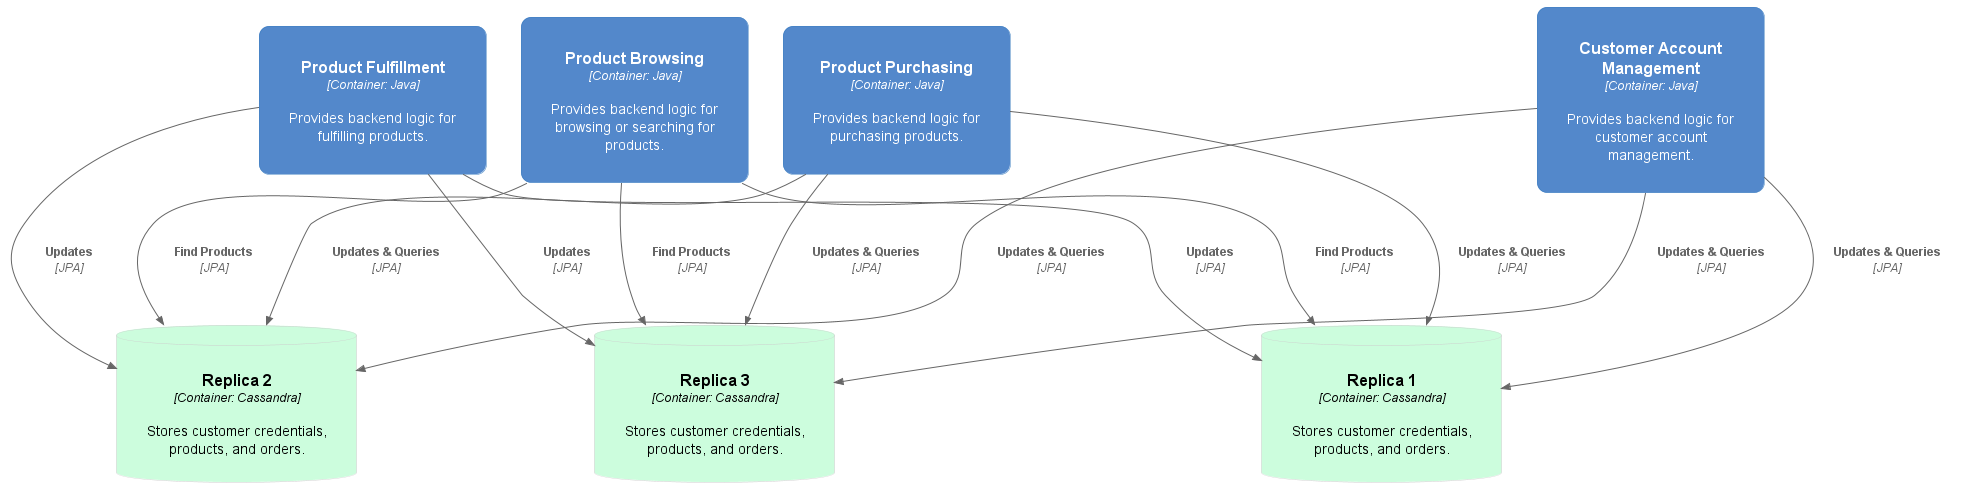
\includegraphics[width=\textwidth]{diagrams/Leaderless}
    \end{center}
    \caption{A leaderless replication of the Sahara database.}
    \label{fig:sahara-leaderless}
\end{figure}

\begin{figure}[ht]
    \begin{center}
    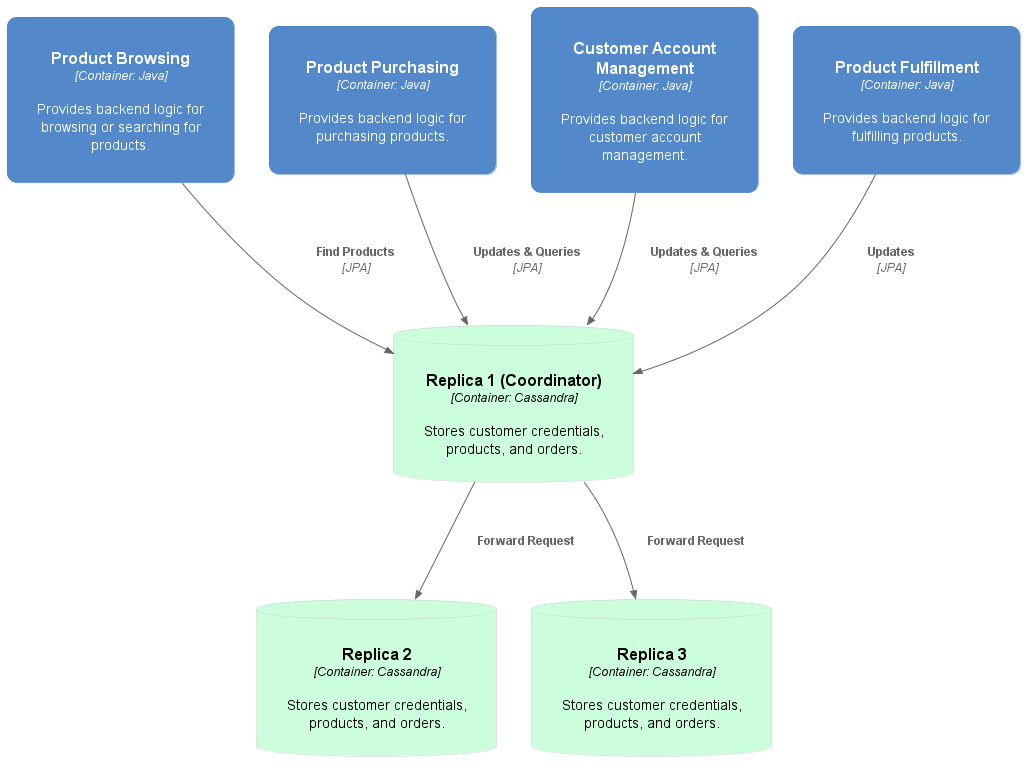
\includegraphics[width=0.6\textwidth]{diagrams/LeaderlessCoordinator}
    \end{center}
    \caption{A leaderless replication using a coordinator node of the Sahara database.}
    \label{fig:sahara-leaderless-coordinator}
\end{figure}

In leaderless databases,
any database node may go offline at any point and the system should continue to function, assuming only a few nodes go offline.
This type of database gives us excellent reliability and scalability as we can keep adding extra replicas to increase our capacity.
But how can we support this?

\subsubsection*{Quorum}

To support the extensibility of leaderless databases,
we need to duplicate our read and write requests.
As a simple example,
take Figure \ref{fig:sahara-leaderless},
we have three replicas of our database.
When making a write request,
if we send our write to just one replica then at most two replicas can have outdated data.
Therefore when we read, we need to read from all three replicas to ensure one will have the most recent writes.
If instead,
we write to two replicas then at most one replica will have outdated data.
Then we need only read from two replicas to ensure that at least one will have the most recent writes.

To generalise, if we have a leaderless database of $n$ replicas,
we need to satisfy that,
$$
w + r > n
$$
where $w$ is the amount of replicas to write to and $r$ is the amount of replicas to read from.
By satisfying this equation we have quorum consistency,
the set of writes and reads must overlap,
which means that reading stale data is \textsl{unlikely}%
\footnote{The cases where stale data can still be read are enumerated in M. Kleppmann \cite{data-intensive}.}.

\section{Partitioning}

Partitioning involves distributing the contents of a database across multiple nodes.
It differs from replication as nodes do not store complete copies of the database.
Often partitioning is combined with replication to prevent the lost of data if one of the partitions fails.
Partitioning is required when we have a large amount of data to store.

When we start partitioning data onto multiple nodes,
we need to consider how we decide which data belongs to which node.
There are two primary approaches to this decision.

\subsection*{Partition by Key Range}
We assume that data is given a key,
with a key-value database this is required,
in relational databases the schema should specify a primary key column.
One approach to partitioning is to divide the range of key values and partition based on that.
Consider the UQ student database,
the key would be the student ID.
We can then partition the database based on student ID,
say all student numbers between \texttt{s0000000} and \texttt{s1000000} are stored on partition 0,
all numbers between \texttt{s1000001} and \texttt{s2000000} are stored on partition 1, etc.

This approach appears practical,
each partition has an equal share of database entires.
However, as time goes on certain partitions become less used while others become very popular.
We might imagine that at the moment,
partitions 5 and 6 would be used far more frequently than partition 0.
This is known as \textsl{skewed partitioning}.

\subsection*{Partition by Hash}

Consider hash maps,
we use hashes of the keys to allocate values into buckets.
A good hashing algorithm minimizes the amount of collision (a value stored in the same bucket).
We can apply the same process to database partitioning,
hashing the key of a record allows us to maximize the spread of partition usage.
The disadvantage of partitioning by hash is that only queries by key are efficient,
queries by ranges of keys are no longer efficient as they require \emph{all} partitions to be queried.%
\footnote{Databases such as Cassandra use compound primary keys to help resolve this issue.}

\subsection*{Secondary Indices}

Databases often rely on secondary index to perform a range of useful queries.
In our UQ student database example,
a database field which is often useful to query might be the degree of a student record.
We might want this query to run efficiently as schools could need to frequently query for these collections to implement their own services.

The two approaches to this are local or global indices.
With local indices, each partition stores an index for their own partition of the data.
With global indices, a partition is assigned to manage a particular secondary index value.
For example, partition 2 might store the index for all Bachelor of Software Engineering students.

Local indices allow efficient writing,
as a write only has to update the index of the partition to which it is writing.
However, it introduces slower reads as all partitions must be queried for their index.
Global indices slow down writing as all relevant partitions need to have their partition updated.
Although it can increase read speeds as a query only needs to look at the relevant partitions.

\subsection{Rebalancing}

Over time some partitions may get more frequent use than others.
We might also add or remove nodes.
This can require the data to be rebalanced to update the range of values stored on any partition.
Rebalancing can be an automated or a manual process.
It is important to consider the effects of rebalancing automatically as they are costly operations
and if triggered at an inappropriate time they can greatly impact the performance of a database.

\subsection{Routing}

Much like auto-scaled stateless services,
we need a way to route traffic that is fair.
However, unlike stateless services,
only one node of the system is capable of processing our request.
We need a mechanism for choosing the appropriate node to which our request is sent.

We might implement a naive load balancer which just balances the load regardless of the request.
This load balancer is will send requests to the wrong nodes.
In such a system, it is the responsibility of the node to forward the request to the node which is capable of answering the query.

A more sophisticated solution would be to deploy a load balancer which is request aware.
This load balancer can forward requests to the appropriate node.

Finally, we might offload the problem to the client.
Requiring that our database clients are aware of how to map their query to the appropriate node.

\section{Transactions}

All of the various failure cases and considerations when working with scalable databases can be overwhelming.
The complexities of distributed databases make reasoning about the logic of an application challenging,
which in turn leads to more bugs and faults.
Fortunately, database developers have a technique to assist in this complexity and allow us to reason about our interactions with the database, \textsl{transactions}.

Transactions bundle related groups of read/write operations together and guarantee useful properties.
Traditionally, these properties are referred to as ACID properties, Atomicity, Consistency, Isolation, and Durability.

\subsection{Atomicity}
Atomicity guarantees that when performing multiple operations,
if one operation cannot be completed successfully then the effects of all operations are aborted.
For example, consider the purchasing process.
When purchasing a product we may wish to both update the stock of the product and reduce the funds of a customer's account.
If either of those operations occurred on their own,
someone would be very unhappy.
Atomicity guarantees that either all operations in a transaction succeed or none do.

\subsection{Consistency}
Consistency guarantees that any application specific invariants of the database are preserved by transactions.
For example, we might introduce the invariant that the stock of an item cannot be below zero.
This invariant must then be maintained by all transactions.

\subsection{Isolation}
Isolation allows transactions to pretend that they are the only operation performing on the data.
Transactions appear to preform sequentially even though they may in reality be performing concurrently.
This allows transactions to ignore a whole host of issues related to concurrency.

\subsection{Durability}
Durability provides a guarantee that once transactions are completed,
their updates are preserved.
In distributed databases this is often an assurance that the updated data has been copied to other machines.

\section{Conclusion}

Scaling out services that have persistent data requires far greater care than stateless services.
We have seen approaches for coping with undue load on individual nodes via replication.
We have seen approaches for handling greater volume of data than can be stored on a single machine via partitioning.
We have noted that often one might want to combine the approaches of replication and partitioning for the one database system.
Both of these techniques introduce a new range of complexity for programmers to deal with.
In our final section we briefly introduced how transactions, and the guarantees they provide, can help developers in reasoning about their database interactions.

This lecture note has been a very brief introduction into the topics of replication, partitioning, and transactions.
The content has been structured around the Chapters 5, 6, and 7 of \textit{Designing Data-Intensive Applications} \cite{data-intensive}.
You are strongly encouraged to read these chapters of the book for a much more in-depth look at all of the topics covered.
